\documentclass[11pt, oneside]{article} 
\usepackage{geometry}
\geometry{letterpaper} 
\usepackage{graphicx}
	
\usepackage{amssymb}
\usepackage{amsmath}
\usepackage{parskip}
\usepackage{color}
\usepackage{hyperref}

\graphicspath{{/Users/telliott_admin/Tex/png/}}
% \begin{center} 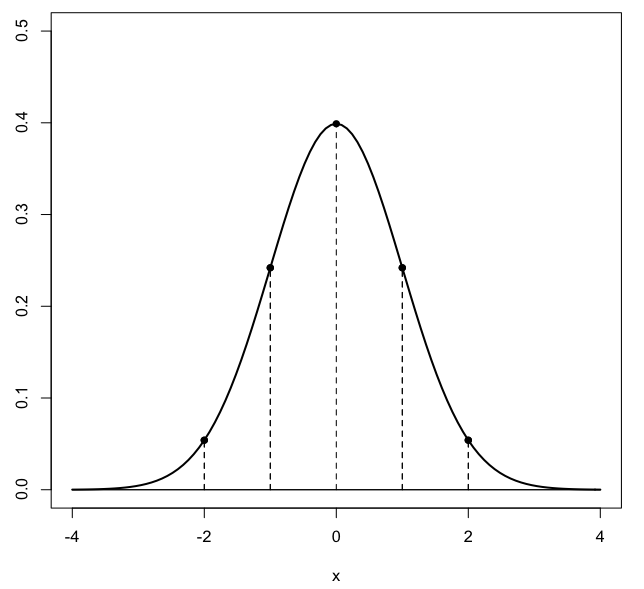
\includegraphics [scale=0.4] {gauss3.png} \end{center}

%break
\title{Differential}
\date{}

\begin{document}
\maketitle
\Large

\subsection*{infinitesimals}
We say that the derivative $dy/dx$ is the slope of the tangent to the curve $y = f(x)$ at some particular point $(x,y)$;  it is the slope of a line that just touches the curve.

And it is frequently called the slope of the curve at the point $(x,y)$.

We saw a formal definition for the derivative in terms of an expression for $\Delta y$ as a function of $\Delta x$, which is then divided by $\Delta x$.  We determine what is called the "limit" as $\Delta x$ approaches zero.
\[ \frac{dy}{dx} = \lim_{\Delta x \rightarrow 0} \frac{\Delta y}{\Delta x} \]

There appears to be a contradiction here.  On one hand, we're saying that $\Delta x$ must approach zero.  On the other hand, it cannot really be zero, because division by zero is not defined.  So how close does it have to be to zero?  

Are $dy$ and $dx$ small, really small, really really small, or almost zero?  

The official answer requires a cumbersome apparatus of limits, and it would say that $dy/dx$ is not a quotient at all, but rather a single entity, the limit of a quotient, as we just said:
\[ \frac{dy}{dx} = \lim_{\Delta x \rightarrow 0} \frac{\Delta y}{\Delta x} \]

However, our simple answer is that $dx$ and $dy$ are separable entities and they are just as small as they need to be.  Take the example we used previously:
 \[ \frac{dy}{dx} = 3cx^2 \]
Put the $dx$ on the right-hand side:
\[ dy = 3cx^2 \ dx \]

What this expression says is that for a small change in $x$ which we call $dx$, we will obtain a small change in $y$ called $dy$ with the given relationship.  $3cx^2$ gives the proportionality between $dx$ and $dy$.

Suppose we evaluate $3cx^2$ at some particular $x_0$.  Then it is a number, it has a fixed value depending on where we are on the curve.  So write it as $k = 3cx_0^2$ and then:
\[ dy = k \ dx \]
When we write this, we are making a \emph{linear approximation} to the quadratic function.  $dy$ is not exactly equal to $k \ dx$, for most situations we are ignoring quadratic and higher terms.

Here, we treat $dy$ and $dx$ as very small but non-zero quantities.  If there should ever be a problem because we've chosen $\Delta x$ too large, just reduce it by some factor ($1/10$, $10^{-6}$, $1/$googol), whatever is needed,

\url{https://en.wikipedia.org/wiki/Googol}

and try again until the problem disappears (it will).  Make $dx$ and $dy$ really really small.  If that's not small enough, try making them smaller still.

By this trick, we free ourselves from limits.  If you want to multiply by $dx$ on both sides of an equality
\[ \frac{dy}{dx} = n x^{n-1} \]
\[ dx \cdot \frac{dy}{dx} = dy = n x^{n-1} \ dx \]
Feel free, go ahead and do it.

\subsection*{fancy}

If you want to read more about the derivative as a limit, why $dy/dx$ is not a quotient, and so on, you can look at any standard calculus book.  Or start here

\url{https://math.stackexchange.com/questions/21199/is-frac-textrmdy-textrmdx-not-a-ratio}

The bottom line is that we want $dy$ and $dx$ to be very small compared to $y$ and $x$, but one of the properties of the real numbers is that no matter how small small we choose $A$ (or $dx$), there exists a positive integer $n$ such that $n \cdot A > B$ (or $n \cdot dx > x$).  This is called the Archimedean property of the real numbers.
\begin{center} 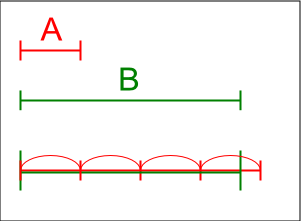
\includegraphics [scale=0.6] {Archimedean_property.png} \end{center}

Effectively what limits and neighborhoods do is to say, OK smart guy, you go first.  Pick $n$.  Then once you've picked $n$ very large, we can always find $dx$ very very small so that $n \cdot dx$ is still small compared with $x$.  That's the whole trick.

However, in practice none of this is a problem because we view $dy$ and $dx$ as very small.  Although often we only care about their ratio, some times we will need to separate them.  This is legal, trust me.

\end{document}